Here is a basic example. I give you some arbitrary $z, w > 0$. Can you find a unique $x, y \in \Real$ such that $z = x + y$ and $w = xy$? The first observation we might make is that it seems unlikely that we even can find real solutions. For example, consider $z = \frac{1}{2}$ and $w = 1$. Then a solution $(x, y)$ would correspond to an intersection of graphs in the image below:

\begin{figure}[h]
	\centering
	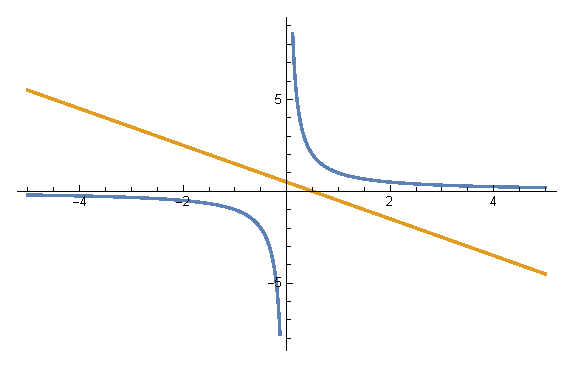
\includegraphics{plots_gr3.eps}
	\caption{Graphs of $x + y = 1/2$ and $xy = 1$}
	\label{fig:plots_gr3}
\end{figure}

and clearly there are no intersections. Moreover, if we have a solution, it will very likely not be unique. This is because if $(x, y)$ solves the system above, so does $(y, x)$ because of the commutativity of addition and multiplication.

How does this even relate to the inverse function theorem? Define $F(x, y) = (x + y, xy)$. Clearly $F$ is $\CD{1}$, with
\[DF(x_0, y_0) = \begin{bmatrix} 1 & 1 \\ y_0 & x_0\end{bmatrix}.\] Then $DF(x_0, y_0)$ is invertible if and only if $x_0 - y_0 \neq 0$. This sort of matches our remarks from earlier: since when $x = y$ we can see that near the intersection point we have local non-invertibility of the function $F$ in question.

Now suppose $x_0 \neq y_0$. Then the inverse function theorem tells us that in some neighborhood $V$ of $(x_0, y_0)$ there exists a bijective mapping $f|V$. So locally there is a solution for $f(x_0, y_0)$. But this doesn't answer our original question: what exactly can $z$ and $w$ be?

Fortunately, or not, we can kill this with elementary observations. The quadratic equation $x^2 -zx + w$ has roots $x$ and $y$. So $x$ and $y$ are real only if 
\[\sqrt{w^2 - 4z} \geq 0 \implies z \leq \frac{w^2}{4}.\]

